\documentclass{article}%
\usepackage{amsmath}
\usepackage{amsfonts}
\usepackage{amssymb}
\usepackage{graphicx}
\usepackage{tikz}
\usepackage{hyperref}%
\setcounter{MaxMatrixCols}{30}
%TCIDATA{OutputFilter=late$x2$.dll}
%TCIDATA{Version=5.00.0.2552}
%TCIDATA{CSTFile=40 LaTeX article.cst}
%TCIDATA{Created=Thursday, August 21, 2008 14:03:59}
%TCIDATA{LastRevised=Wednesday, October 01, 2014 12:46:33}
%TCIDATA{<META NAME="GraphicsSave" CONTENT="32">}
%TCIDATA{<META NAME="SaveForMode" CONTENT="1">}
%TCIDATA{<META NAME="DocumentShell" CONTENT="Standard LaTeX\Blank - Standard LaTeX Article">}
%TCIDATA{Language=American English}
\newtheorem{theorem}{Theorem}
\newtheorem{acknowledgement}[theorem]{Acknowledgement}
\newtheorem{algorithm}[theorem]{Algorithm}
\newtheorem{axiom}[theorem]{Axiom}
\newtheorem{case}[theorem]{Case}
\newtheorem{claim}[theorem]{Claim}
\newtheorem{conclusion}[theorem]{Conclusion}
\newtheorem{condition}[theorem]{Condition}
\newtheorem{conjecture}[theorem]{Conjecture}
\newtheorem{corollary}[theorem]{Corollary}
\newtheorem{criterion}[theorem]{Criterion}
\newtheorem{definition}[theorem]{Definition}
\newtheorem{example}[theorem]{Example}
\newtheorem{exercise}[theorem]{Exercise}
\newtheorem{lemma}[theorem]{Lemma}
\newtheorem{notation}[theorem]{Notation}
\newtheorem{problem}[theorem]{Problem}
\newtheorem{proposition}[theorem]{Proposition}
\newtheorem{remark}[theorem]{Remark}
\newtheorem{solution}[theorem]{Solution}
\newtheorem{summary}[theorem]{Summary}
\newenvironment{proof}[1][Proof]{\noindent\textbf{#1.} }{\ \rule{0.5em}{0.5em}}

\usepackage{fancyhdr}
\setlength\headheight{26pt}
\pagestyle{fancy}
\lhead{{\footnotesize Light Absorbance for Dyes}}
\rhead{{\footnotesize Christopher Chapline}}
\begin{document}

\begin{center}

    \section*{Tabular Data}

    \begin{tabular}{| l | l | l | l | l |}
        \hline
        & Blue  & Green  & Red  \\ \hline
        400         & 0.02  & 0.85  & 0.19  \\ \hline
        450         & 0     & 0.65  & 0.28  \\ \hline
        500         & 0.04  & 0.09  & 0.58  \\ \hline
        550         & 0.19  & 0.2   & 0.26  \\ \hline
        600         & 0.75  & 0.7   & 0.02  \\ \hline
        650         & 0.95  & 0.85  & 0     \\ \hline
    \end{tabular}

    \vspace{10mm}

    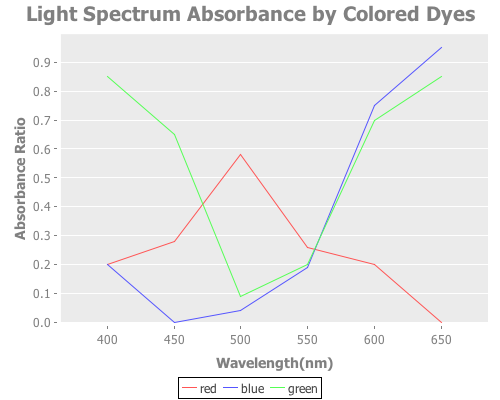
\includegraphics[width=0.8\textwidth]{./charts/absorbance.png}
\end{center}

\end{document}
